\documentclass{liu_mall}
\usepackage{comment}
\newcommand{\version}{Version 1.2}
\author{Dennis Abrikossov, \url{denab905@student.liu.se}\\
  Philip Bromander, \url{phibr608@student.liu.se}}
\title{Systemdokumentation}
\date{2023-10-12}
\rhead{Dennis Abrikossov\\
Philip Bromander}

\begin{document}
    \projectpage
    \section{Revisionshistorik}
        \begin{table}[!h]
            \begin{tabularx}{\linewidth}{|l|X|l|}
                \hline
                Ver. & Revisionsbeskrivning & Datum \\\hline
                1.2 & Modifierade dokumentet för en första inlämning & 12/10/23\\\hline
                1.1 & Modifierade dokumentet för att hålla tabeller istället & 05/09/23\\\hline
                1.0 & Fyllt i dokument med deadlines \& veckor & 01/09/23\\\hline
            \end{tabularx}
        \end{table}

    \newpage
    \rowcolors{1}{LightGray}{Silver}
    \section{Flödesdiagram}
        I figur \ref{fig:Data Flow Diagram} kan vi observera flödesdiagrammet för det aktuella systemet.
        \begin{figure}[h!]
            \centering
            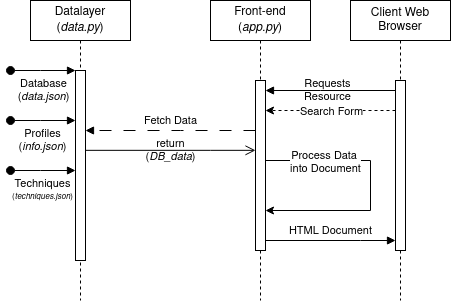
\includegraphics{TDP003 Diagram}
            \caption{Flödesdiagram}
            \label{fig:Data Flow Diagram}
        \end{figure}\\
        När klienten önskar att hämta data initierar den en förfrågan.
        Front-end tar sedan hand om denna förfrågan och ansvarar för att interagera med användaren för att se till att vidare förfrågningar av användaren hanteras korrekt.

        För att uppfylla användarens förfrågan hämtar front-end data från dataregistret via datalagret. Datalagret fungerar som en handhavare för data som behövs för att svara på klientens förfrågan. Här sparas all information och data som systemet behöver medans den hanterar en begäran.
        
        Front-end bearbetar sedan datan datalagret hämtade och formaterade för att utföra ytterligare behandling eller formatering i mån för att skriva ut till en webbläsare som ett HTML-dokument. När front-end har hanterat datan godtyckligt 
        skickar den tillbaka det färdigställda dokumentet till klienten, som ska presentera den till användaren som skapade begäran.
        
        Flödesdiagrammet i figur \ref{fig:Data Flow Diagram} illustrerar hur informationen och datan rör sig genom systemet; från användarens förfrågan till hämtning och bearbetning av data från databasen i datalagret till den slutliga presentationen för klienten. Detta är en översiktlig illustration av hur systemet fungerar. Observera i figur \ref{fig:Specific Use-case Scenario} hur en användare kan söka upp ett specifikt projekt och hur interaktionen handskas mellan användaren, huvudprogrammet, datalagret, och databasen. I figur \ref{fig:Specific Use-case Scenario} börjar användaren med att klicka in sig på söksidan för projekt, antingen med eller utan sökkriterier, och sedan begär att få se ett specifikt projekt efter det att användaren har sett resultaten av sin sökning.
        \begin{figure}
            \centering
            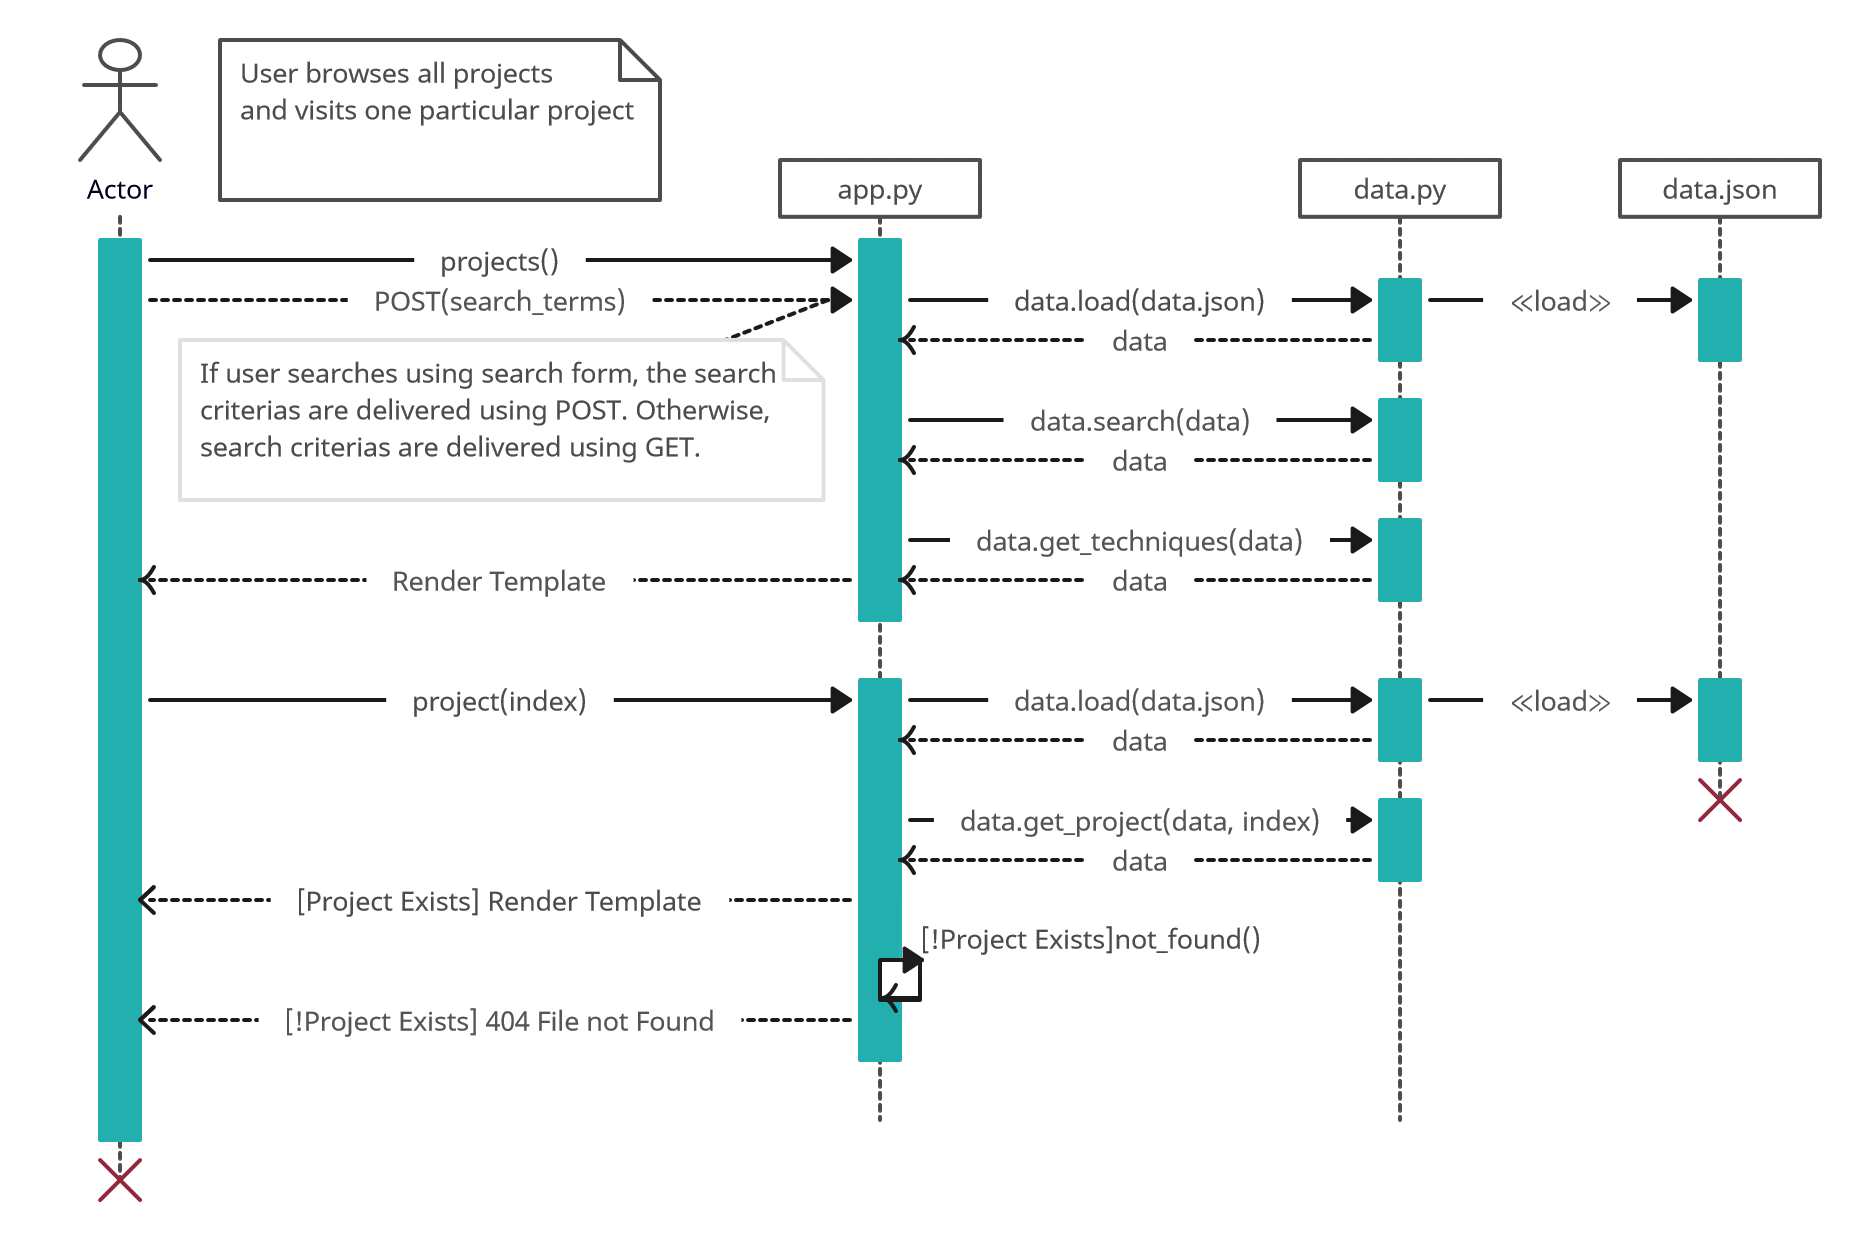
\includegraphics[scale=0.25]{Specific_User_Scenario.png}
            \caption{En användare söker efter ett specifikt projekt}
            \label{fig:Specific Use-case Scenario}
        \end{figure}

    \newpage
    \section{Datalager}
        Följ URL:n för att se API:n för datalagret som erfordrat av Linköpings Universitet:\newline
        \url{https://www.ida.liu.se/~TDP003/current/portfolio-api_python3/data-module.html}
    
        \iffalse % \begin{comment} fungerar inte för vi har inte Verbatim paketet
            Dokumentet är skrivet för att underlätta underhåll av systemets kodbas.\\
            Det skall finnas minst en förklarad översiktsbild.\\ (Klar?)
            Det skall finnas hänvisning till kursens specifikation av datalagret.\\
            Funktioner som ingår i presentationslagret skall vara specificerade i detaljnivå motsvarande datalagrets specifikation. Det finns verktyg för att automatiskt generera denna typ av dokumentation utifrån källkoden (till exempel Epydoc). Det förutsätter förstås att källkoden har korrekt formaterade kommentarer.\\ (Klar?)
            Det skall finnas minst ett sekvensdiagram för en specifik användarsituation.\\
            Det skall finnas ett avsnitt som beskriver hur fel hanteras och loggas, och var utvecklare kan hitta portfoliologgen (finns exempelvis i terminalen). Här ska även finnas en beskrivning av metoder och program som används vid felsökning, speciellt om koden är förberedd för ett specifikt verktyg eller en specifik metod. Under utveckling skapas ofta enhetstester, dokumentera vilka som finns och hur de används (exempelvis de gemensamma testfallen(tester för datalagret)).\\
        
            Bilder/figurer ska ha förklarande figurtexter med nummer, och de ska refereras till i texten.\\
            Det skall finnas information om författare, datum, dokumentversion, projektnamn, kurs och totalt antal sidor (dessa saker är bra att ha med i en dokumentmall, t.ex. i sidhuvud/sidfot på varje sida).\\
            Inlämning sker som pdf med höga krav på språk och tydlig layout. Korrekturläs. Använd flera rubriknivåer. Sätt tydliga relevanta rubriker. Använd bilder och figurer för att förtydliga eller exemplifiera det som beskrivs i text. Numrera figurer och tabeller och hänvisa i texten så bilden ingår i den röda tråden. Formatera konsekvent kod, filnamn, eller andra typer av nyckelord med en annan font. Infoga innehållsförteckning om det är motiverat utifrån sidantalet, färre än fem sidor behöver sällan förteckning, det är lätt hitta ändå.\\
            
            Källkoden ska kommenteras på engelska för varje modul, funktion och för varje global variabel. Ej självförklarande kodavsnitt ska även kom- menteras löpande i koden.\\
            Alla namn på filer, moduler, funktioner och variabler ska vara på eng- elska.\\
            En systemdokumentation ska ingå i systemets dokumentation. En README-fil ska beskriva hur systemet är paketerat och peka ut övrig dokumentation. Tydliga installationsinstruktioner ska ingå, antingen som en del av README-filen eller i valfri annan fil utpekad av README-filen.\\
            En användarmanual ska ingå i systemets dokumentation.\\
            Testerna ska dokumenteras och skall ingå i systemets dokumentation.\\
        \fi
        
    \section{API för presentationlagret}
    \subsection{Funktionsöversikt}
    \begin{table}[!h]
        \begin{tabularx}{\textwidth}{p{5cm}|p{10.65cm}}
            \hline
            \textbf{Function} & Function description\\
            \hline
            \textbf{index()} & Loads information from "info.json" and renders it on the "index.html" page.\\
            \hline
            \textbf{projects()} & Handles project search and sorting based on user input, rendering the results on the "projects.html" page.\\
            \hline
            \textbf{techniques()} & Retrieves statistics on techniques used in projects and displays them on the "techniques.html" page.\\
            \hline
            \textbf{project(index)} &  
            Displays details for a specific project based on its index on the "project.html" page.\\
            \hline
            \textbf{not\_found(err\_message)} &  
            Handles 404 errors by displaying an error message on a custom error page.\\
            \hline
            \textbf{generic\_error(err\_message)} & Handles generic exceptions by displaying an error message on an error page.\\
            \hline
            \textbf{log(level: str,\newline
                    message: str,\newline
                    source: request = "")} &
                    This function is responsible for server logging, recording error messages,
                    warnings, and debugging information, and saving them to a log file.\\
            \hline
        \end{tabularx}
        \label{table:funktions}
    \end{table}
    
    \subsection{Funktionsdetaljer}
    
    \iffalse
    \hline
    \textbf{POST Request:} & Reads form data including sorting options, search parameters, and selected techniques.
        Loads the project database using "data.load".
        Retrieves all techniques used in the database with "data.get\_techniques."
        Searches the database for projects matching the search criteria.
        Renders the "projects.html" template with the search results and selected filters.\\
        \hline
    \textbf{GET Request:}  & Similar to POST but retrieves parameters from the query string. \\

    \textbf{GET Request} & Loads the project database using "data.load".
                    Retrieves project details by index using "data.get\_project".
                    Handles image and content checks, providing fallbacks when necessary.
                    Renders the "project.html" template with project details.\\
            \hline
    \fi
    
    \begin{table}[!h]
        \begin{tabularx}{\textwidth}{p{4.5cm}|p{11.15cm}}
            \hline
            \textbf{index()} &  Loads information from "info.json" using the "data.load" function\newline
                                and renders the "index.html" template with the extracted information\newline
                                as "information\_developers".\\
            \hline
            \textbf{Parameters:} & None \\
            \hline
            \textbf{Return value:}\newline
                Rendered Template Object & A rendered template for the "index.html" page. \\\hline
        \end{tabularx}
    \end{table}
    \vspace{-5mm}
    \begin{table}[!h]
        \begin{tabularx}{\textwidth}{p{4.5cm}|p{11.15cm}}
            \hline
            \textbf{projects()} & Handles GET and POST requests for the /projects route. \\
            \hline
            \textbf{Parameters:} & None\\
            \hline
            \textbf{Return value:}\newline
                Rendered Template Object & A rendered template for the "projects.html" page with search results. \\
            \hline
        \end{tabularx}
    \end{table}
    \vspace{-5mm}
    \begin{table}[!h]
        \begin{tabularx}{\textwidth}{p{4.5cm}|p{11.15cm}}\hline
            \textbf{techniques()} & Loads information from "techniques.json" and "data.json".\newline
                                    Retrieves statistics for techniques used in projects\newline
                                    using "data.get\_technique\_stats".\\
            \hline
            \textbf{Parameters:} & None \\
            \hline
            \textbf{Return value:}\newline
                Rendered Template Object & A rendered template for the "techniques.html" page\newline
                                         with technique information and statistics.\\
            \hline
        \end{tabularx}
    \end{table}
    \vspace{-5mm}
    \begin{table}[!h]
        \begin{tabularx}{\textwidth}{p{4.5cm}|p{11.15cm}}
            \hline
            \textbf{project(index)} & Handles GET requests for individual project details\newline
                                      using the project's index.\\
            \hline
            \textbf{Parameters:} &\\
                index: int & The index of the requested project.\\ 
            \hline
            \textbf{Return value:} &\\
                Rendered Template Object & A rendered template for the "project.html" page with project details.\\
            \hline
        \end{tabularx}
    \end{table}
    \vspace{-5mm}
    \begin{table}[!h]
        \begin{tabularx}{\textwidth}{p{4.5cm}|p{11.15cm}}\hline
            \textbf{not\_found\newline
                (err\_message)} & Handles 404 errors by rendering an error page with a provided error message and a custom image.\\\hline
            \textbf{Parameters:} &\\
                err\_message: str & The error message to display.\\\hline
            \textbf{Return value:} &\\
                Rendered Template Object & A rendered error template with the error message and image.\\
            \hline
        \end{tabularx}
    \end{table}
    \vspace{-5mm}
    \begin{table}[!h]
        \begin{tabularx}{\textwidth}{p{4.5cm}|p{11.15cm}}\hline
            \textbf{generic\_error\newline
                (err\_message)} &   Handles generic exceptions by rendering an error page\newline
                                    with a provided error message.\\
            \hline
            \textbf{Parameters:} &\\
                err\_message: str & The error message to display.\\ 
            \hline
            \textbf{Return value:} &\\
                Rendered Template Object & A rendered error template with the error message.\\
            \hline
        \end{tabularx}
    \end{table}
    \vspace{-5mm}
    \begin{table}[!h]
        \begin{tabularx}{\textwidth}{p{4.5cm}|p{11.15cm}}
            \hline
            \textbf{log(level: str,\newline
            message: str,\newline
            source: request = "")} &
            This function is responsible for server logging, recording error messages,\newline
            warnings, and debugging information, and saving them to a log file.\\\hline
            \textbf{Parameters:}&\\
            level: str & A fully capitalized string indicating the error level.\\
            message: str & A string literal containing the log message\\
            source: request = "" & The connection metadata (primarily for fetching IP).\\\hline
            \textbf{Return value:} & None\\
            \hline
        \end{tabularx}
        \label{table:log()}
    \end{table}
    
    \newpage
    \section{Felhantering och loggning}
        \subsection{Felhantering}
            Om det uppstår ett fel i systemet medans det arbetar måste det hanteras på ett godtyckligt sätt så att inte förhindra servern ifrån att hantera nya förfrågningar. Detta hanterar systemet med enkel felhantering. Det finns två källor till problem: om Flask blir tillsagd att producera en sida som inte existerar, och om datalagret får en förfrågan som den inte kan hantera. Det första fallet är enkelt att hantera med en 404 ("not found") felkod. Får Flask en förfrågan om en undersida som inte existerar skickar den användaren till en speciell 404-felsida.
    
            Den andra källan till fel är svårare att hantera godtyckligt eftersom systemet kan inte förutspå alla sätt datalagret kan misslyckas. Detta måste man hitta och underhålla genom att testa systemet. Ett fall som var under utvecklingen en källa till fel var när sökfunktionen fick en sträng som maskerades som en del av ett reguljärt uttryck och sökfunktionen blev förvirrad över hur den skulle söka. Detta är inte längre ett problem.

        \subsection{Loggning}
            För att hantera systemet i framtiden är det viktigt att veta vad som händer i systemet medans det körs och att kunna gå tillbaka i tiden för att läsa äldre felmeddelanden. Detta görs genom ett loggningsystem. I källkoden hanterar en funktion med namnet 'log' detta. Den skriver både ut i realtid felmeddelanden färgkodade i terminalen och skriver samtidigt ner felmeddelanden till en fil med namnet 'log.md'. Logfilen är placerad tillsammans med huvudprogrammet och innehåller en lista av meddelanden, komplett med datumstämpel, felnivå, IP-address, och meddelande. Felnivå berättar hur allvarligt meddelandet är och kommer i fyra klasser: 'DEBUG' för användning under utveckling, 'INFO' för ofarliga körmeddelande, 'WARNING' för de mestadels ofarliga felmeddelanden, och 'ERROR' för de mest kritiska felmeddelanden.

    \section{Enhetstester}
        För att säkerställa att systemet fungerar som det ska under alla oförutserbara körsätt måste man testa programvaran. Det mest konkreta sättet att utföra detta på är genom enhetstester. För projektet var enhetstesterna för datalagret givna; dessa tester ser till att den mest grundläggande funktionaliteten fungerar. Till exempel testas'load'-funktionen om den laddar projekten rätt och är i korrekt ordning, vilket måste säkerställas manuellt. Den kollar också om det går att söka på ett ord med flera sökfält aktiverade samtidigt. Den testar däremot inte när man söker på flera tekniker samtidigt, om det kommer upp projekt som har alla markerade tekniker och inte bara första bästa.
\end{document}